\chapter{Struna gitary i alikwoty}\label{rozdz:alikwoty}

\section{Dlaczego nuta to nie jedna sinusoida?}

Gdy zagramy na gitarze nutę A2, w nagraniu nie ma jednej sinusoidy $110\Hz$. Jest cały szereg sinusoid:
$110$, $220$, $330$, $440$\dots\ Hz. Te dodatkowe składowe nazywamy \emph{alikwotami} (harmonicznymi).
To one nadają instrumentowi barwę, ale też sprawiają największy kłopot w transkrypcji: alikwoty jednej nuty
lądują dokładnie tam, gdzie leżą \emph{inne} nuty. Ten rozdział wyjaśnia, skąd się biorą i dlaczego
na osi logarytmicznej wyglądają jak niezmienny wzorzec --- na tym wzorcu opiera się pierwszy blok sieci Gen~6.

Po tym rozdziale umiesz: (i)~uzasadnić, że struna drga z częstotliwościami $kf_0$, (ii)~wskazać, które nuty
dzielą alikwoty, (iii)~policzyć położenie $h$-tego alikwotu w półtonach i binach, (iv)~wyjaśnić, skąd bierze się
błąd oktawowy.

\section{Drgania własne struny}

Struna o długości $L$ jest zamocowana na obu końcach. Jej wychylenie $u(x,t)$ w punkcie $x\in[0,L]$ i chwili $t$
spełnia równanie falowe $u_{tt}=v^2u_{xx}$, gdzie $v$ to prędkość fali na strunie (zależy od naciągu i masy),
oraz warunki brzegowe $u(0,t)=u(L,t)=0$.

\haslo{fala stojąca}
\begin{definicja}[Fala stojąca (tryb własny)]\label{def:fala-stojaca}
\emph{Falą stojącą} nazywamy rozwiązanie równania falowego postaci $u(x,t)=\phi(x)\cos(2\pi ft)$, w którym
kształt $\phi(x)$ nie zmienia się w czasie, tylko jego wychylenie pulsuje z częstotliwością $f$.
\end{definicja}

\begin{twierdzenie}[Częstotliwości własne struny]\label{tw:struna}
Funkcje
\[u_k(x,t)=\sin\!\Big(\frac{k\pi x}{L}\Big)\cos(2\pi f_k t),\qquad k=1,2,3,\dots,\]
są falami stojącymi spełniającymi równanie falowe i warunki brzegowe wtedy i tylko wtedy, gdy
\begin{equation}
  f_k = k\,\frac{v}{2L}=k f_1 .
\end{equation}
\end{twierdzenie}
\begin{pomyslDowodu}
Wstawiamy $u_k$ do równania $u_{tt}=v^2u_{xx}$, policzymy obie drugie pochodne i porównamy współczynniki.
\end{pomyslDowodu}
\begin{proof}
Warunki brzegowe są spełnione, bo $\sin(0)=0$ oraz $\sin(k\pi)=0$ dla całkowitego $k$. Liczymy pochodne (wzory
$(\sin ax)''=-a^2\sin ax$ i $(\cos bt)''=-b^2\cos bt$ są znane ze szkoły):
\begin{align*}
u_{tt} &= -(2\pi f_k)^2\,u_k, && \pow{(po czasie)}\\
u_{xx} &= -\big(\tfrac{k\pi}{L}\big)^2u_k. && \pow{(po położeniu)}
\end{align*}
Równanie $u_{tt}=v^2u_{xx}$ jest więc równoważne $(2\pi f_k)^2=v^2(k\pi/L)^2$, czyli $2\pi f_k=vk\pi/L$, skąd
$f_k=kv/(2L)$ (bierzemy dodatni pierwiastek, bo $f_k>0$). Dla dowolnego innego $f$ równość nie zachodzi, więc
$f=f_k$ jest warunkiem koniecznym i wystarczającym. Struna może więc drgać z częstotliwościami będącymi całkowitymi
wielokrotnościami najniższej z nich. To kończy dowód.
\end{proof}

Że \emph{każde} drganie struny jest sumą takich fal, orzekł Daniel Bernoulli (rozwinięcie w szereg Fouriera; dowód
wykracza poza zakres tej książki). Dlatego nuta gitary to suma sinusoid:
\begin{equation}
  x(t)=\sum_{h=1}^{H}A_h\sin\big(2\pi\,h f_0\,t+\varphi_h\big),\qquad f_0=f_1,
  \label{eq:szereg-harm}
\end{equation}
gdzie $f_0$ nazywamy \emph{częstotliwością podstawową}, a składową $h=2,3,\dots$ \emph{alikwotem} (dokładnie:
$h$-tą \emph{harmoniczną}). Amplitudy $A_h$ zwykle maleją z $h$, ale nie znikają.

\begin{przyklad}[Najniższa struna]\label{prz:alik-e2}
Struna E2 ($f_0=82{,}41\Hz$) ma długość drgającą $L\approx0{,}65\,$m. Z tw.~\ref{tw:struna} prędkość fali to
$v=2Lf_0\approx 2\cdot0{,}65\cdot82{,}41=107{,}1$~m/s. Alikwoty $h=1,\dots,6$ mają częstotliwości
$82{,}4;\ 164{,}8;\ 247{,}2;\ 329{,}6;\ 412{,}0;\ 494{,}4\Hz$. Alikwot $h=4$ ($329{,}6\Hz$) to dokładnie
częstotliwość nuty E4 --- najwyższej, otwartej struny.
\end{przyklad}

\begin{intuicja}
Struna może drgać jako całość ($k=1$), w dwóch połowach ($k=2$), w trzech trzecich ($k=3$) itd. Każdy sposób
ma swoją częstotliwość i wszystkie występują naraz. Szarpnięcie w środku wzbudza głównie nieparzyste, przy
końcu struny --- bogatszy zestaw.
\end{intuicja}

\begin{pulapka}
Prawdziwa struna jest sztywna, więc jej alikwoty są \emph{nieco wyższe} niż $hf_0$:
$f_h\approx hf_0\sqrt{1+Bh^2}$, gdzie $B\ge0$ to współczynnik nieharmoniczności. Dla $B=10^{-4}$ szósty alikwot
jest za wysoki o $1200\log_2\sqrt{1+36\cdot10^{-4}}\approx3{,}1$ centa, a dla $B=10^{-3}$ o $30{,}6$ centa, prawie cały
bin. Dlatego blok harmoniczny w rozdziale~\ref{rozdz:architektura} ma dodatkowy filtr po sąsiednich binach.
\end{pulapka}

\section{Wspólne alikwoty: skąd błąd oktawowy}

\begin{twierdzenie}[Alikwoty oktawy]\label{tw:oktawa-alik}
Niech nuta $A$ ma częstotliwość podstawową $f_0$, a nuta $B$ częstotliwość $2f_0$ (oktawa wyżej). Wtedy każdy
alikwot nuty $B$ jest alikwotem nuty $A$: $h\cdot 2f_0=(2h)\,f_0$. Odwrotnie nie: nieparzyste alikwoty $A$ nie
są alikwotami $B$.
\end{twierdzenie}
\begin{pomyslDowodu}
Wystarczy przepisać $h\cdot2f_0$ jako $(2h)f_0$ i zauważyć, że $2h$ jest całkowite i parzyste.
\end{pomyslDowodu}
\begin{proof}
Niech $h\in\{1,2,\dots\}$.
\begin{align*}
h\cdot(2f_0) &= (2h)\cdot f_0 && \pow{(łączność mnożenia)}
\end{align*}
Liczba $2h$ jest całkowita, więc $(2h)f_0$ to $2h$-ty alikwot nuty $A$. Natomiast $3f_0$ ($h=3$ dla $A$) byłoby
alikwotem $B$ tylko dla $h'$ spełniającego $h'\cdot2f_0=3f_0$, czyli $h'=1{,}5\notin\mathbb N$. Zatem parzyste
alikwoty $A$ pokrywają się z alikwotami $B$, a nieparzyste nie. To kończy dowód.
\end{proof}

W zwykłym języku: gdy gra E3, w widmie jest wszystko, co zgłosiłoby E2 --- z wyjątkiem co drugiego prążka. A skoro
wyższe alikwoty bywają słabe, E3 do złudzenia przypomina E2 z wyciszonym podstawowym tonem. To jest
\emph{błąd oktawowy}: najtrudniejsza pomyłka w transkrypcji gitary (w naszych pomiarach ok. $24\%$ fałszywych
alarmów klatkowych leży dokładnie oktawę od prawdziwej nuty).

\begin{figure*}[ht]
\centering
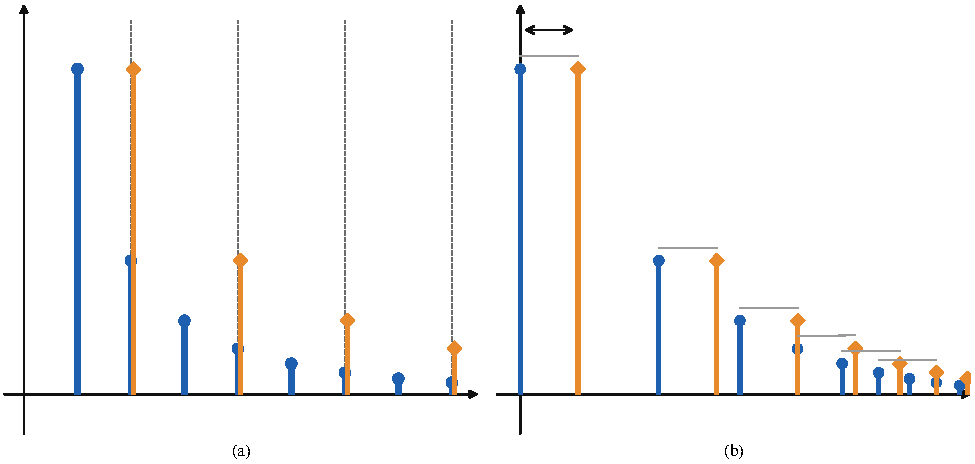
\includegraphics[width=\linewidth]{figures/szereg-alikwotow.pdf}
\caption{Widma szarpniętych strun liczone FFT (wysokość słupka --- amplituda względem prążka podstawowego). (a) Oś liniowa: prążki E2 (niebieskie kółka) i pierwsze cztery prążki E3 (pomarańczowe romby, przesunięte nieco w prawo, żeby były widoczne). Szare przerywane pionowe prowadnice stoją na parzystych prążkach E2: każdy prążek E3 trafia dokładnie w jedną z nich (tw.~\ref{tw:oktawa-alik}).
(b) Oś w półtonach $12\log_2(f/f_{E2})$: wzorzec prążków E2 (niebieskie) i A2 (pomarańczowe) to ta sama figura przesunięta o 5 półtonów (strzałka u góry); cienkie szare łączniki spinają te same numery alikwotów. Kształt zależy tylko od numeru alikwotu, nie od wysokości.}
\label{rys:szereg}
\end{figure*}

\section{Oś logarytmiczna: wzorzec, który się nie zmienia}

Teraz najważniejsze twierdzenie rozdziału. Zmierzmy położenie na osi w półtonach względem ustalonej nuty
odniesienia (np.\ $f_\mathrm{ref}=440\Hz$): $u(f)=12\log_2(f/f_\mathrm{ref})$.

\begin{twierdzenie}[Niezmienniczość wzorca alikwotów]\label{tw:wzorzec}
Jeśli nuta ma częstotliwość podstawową $f_0$ i położenie $u_0=u(f_0)$, to jej $h$-ty alikwot leży w punkcie
\begin{equation}
  u(hf_0)=u_0+12\log_2 h .
\end{equation}
Przesunięcie $12\log_2 h$ zależy od $h$, ale \emph{nie} zależy od $f_0$.
\end{twierdzenie}
\begin{pomyslDowodu}
Logarytm iloczynu jest sumą logarytmów (tw.~\ref{tw:log-iloczynu}): mnożenie przez $h$ staje się dodaniem stałej.
\end{pomyslDowodu}
\begin{proof}
\begin{align*}
u(hf_0) &= 12\log_2\frac{hf_0}{f_\mathrm{ref}} && \pow{(definicja $u$)}\\
        &= 12\log_2 h+12\log_2\frac{f_0}{f_\mathrm{ref}} && \pow{(tw.~\ref{tw:log-iloczynu})}\\
        &= 12\log_2 h+u_0. && \pow{(definicja $u_0$)}
\end{align*}
Stała $12\log_2 h$ nie zawiera $f_0$, więc wzorzec alikwotów ma na tej osi ten sam kształt dla każdej nuty
(rys.~\ref{rys:szereg}b). To kończy dowód.
\end{proof}

\begin{wniosek}[Biny alikwotów]\label{wn:biny}
Przy $3$ binach na półton alikwot $h$ leży o $k_h=36\log_2 h$ binów od podstawy. Zaokrąglone wartości dla
alikwotów używanych w Gen~6:
\begin{center}\small
\begin{tabular}{@{}lccccccc@{}}
\toprule
$h$ & $0{,}5$ & $1$ & $2$ & $3$ & $4$ & $5$ & $6$\\
$12\log_2h$ [półtony] & $-12$ & $0$ & $12$ & $19{,}02$ & $24$ & $27{,}86$ & $31{,}02$\\
$k_h=\round(36\log_2h)$ [biny] & $-36$ & $0$ & $36$ & $57$ & $72$ & $84$ & $93$\\
\bottomrule
\end{tabular}
\end{center}
\end{wniosek}
\begin{proof}
Z tw.~\ref{tw:wzorzec} odstęp w półtonach to $12\log_2h$; przy $3$ binach na półton mnożymy przez $3$:
$k_h=36\log_2h$. Wartości w tabeli to $36\log_2 h$: $36$, $57{,}06$, $72$, $83{,}59$, $93{,}06$ zaokrąglone do
najbliższej liczby całkowitej; np.\ $\round(83{,}59)=84$, a $84$ biny to dokładnie $28$ półtonów, czyli nuta temperowana.
Zaokrąglenie przesuwa więc piąty alikwot o $0{,}41$ bina ($13{,}7$ centa), czyli dokładnie o tyle, o ile ten alikwot
jest za niski względem skali temperowanej.
\end{proof}

\begin{naliczbach}
Struna A2 ($110\Hz$) ma piąty alikwot $550\Hz$. Leży on $12\log_2 5=27{,}86$ półtonów nad A2, czyli blisko nuty
o numerze $45+28=73$ (cis$^{\,3}$, $554{,}4\Hz$), ale o $1200\log_2(550/554{,}4)=-13{,}7$ centa niżej. To nie
błąd modelu, tylko fizyka: trzeci i piąty alikwot nigdy nie trafiają dokładnie w temperowaną skalę.
\end{naliczbach}

\section{Salience: jak wygląda błąd oktawowy w liczbach}

Najprostszy detektor wysokości sumuje energię widma w miejscach, gdzie leżałyby alikwoty kandydata:
$\mathrm{sal}(f)=\frac1H\sum_{h=1}^{H}S(hf)$, gdzie $S$ to amplituda widma. Dla prawdziwej nuty wszystkie składniki są duże.
Ale dla kandydata o oktawę niżej, $f/2$, składniki o parzystym $h$ trafiają w alikwoty prawdziwej nuty, więc salience
też jest wysoka (rys.~\ref{rys:salience}).

\begin{figure}[ht]
\centering
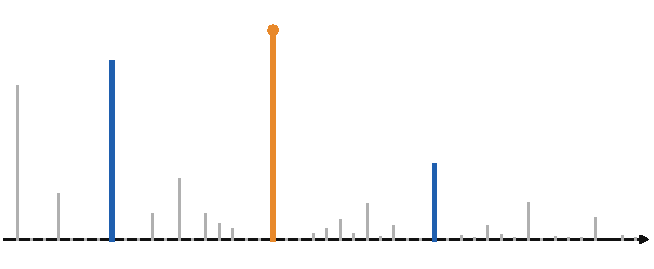
\includegraphics[width=\linewidth]{figures/salience.pdf}
\sidecaption{Salience (suma energii sześciu pierwszych alikwotów, względem największej) dla szarpniętej struny E3 ($m=52$) w funkcji numeru kandydata $m$. Prawdziwa nuta (pomarańczowa) ma najwyższy słupek; pomarańczowa kropkowana pozioma to jej poziom. Kandydat o oktawę niżej ($m=40$, niebieski) jest niewiele niższy, a ten o oktawę wyżej ($m=64$) też się wyróżnia. Szare przerywane pionowe linie to $m=40,52,64$. Wartości liczone z widma FFT jednej nuty. \label{rys:salience}}
\end{figure}

Wniosek praktyczny: samo sumowanie nie wystarcza i trzeba, by sieć porównywała kandydatów \emph{ze sobą}.
Do tego służy uwaga między wysokościami (rozdział~\ref{rozdz:uwaga-wys}).

\section*{Podsumowanie}
\begin{itemize}
\item Struna drga z częstotliwościami $kf_1$ (tw.~\ref{tw:struna}); nuta to suma alikwotów $hf_0$.
\item Prawdziwe struny są lekko nieharmoniczne: $f_h\approx hf_0\sqrt{1+Bh^2}$.
\item Alikwoty nuty o oktawę wyższej zawierają się w alikwotach niższej (tw.~\ref{tw:oktawa-alik}): źródło błędu oktawowego.
\item Na osi półtonów alikwot $h$ leży o $12\log_2h$ nad podstawą, niezależnie od $f_0$ (tw.~\ref{tw:wzorzec}).
\item Przy 3 binach na półton przesunięcia to $-36,0,36,57,72,84,93$ (wn.~\ref{wn:biny}); na nich opiera się blok harmoniczny.
\end{itemize}

\begin{sprawdz}
\begin{enumerate}
\item Wypisz częstotliwości alikwotów $h=1,\dots,8$ struny A2 ($110\Hz$). Które z nich są częstotliwościami podstawowymi nut A3 i E4?
\item Oblicz $12\log_2 7$ i $36\log_2 7$. O ile centów siódmy alikwot odbiega od najbliższej nuty temperowanej?
\item Pokaż, że alikwoty nuty o częstotliwości $3f_0$ (dwunasta wyżej) są alikwotami nuty $f_0$. Które z nich się pokrywają?
\item Struna ma $B=10^{-3}$. O ile centów podwyższony jest alikwot $h=4$? Czy mieści się w jednym binie ($33{,}3$ centa)?
\end{enumerate}
\end{sprawdz}

\subsection*{Rozwiązania}
\begin{enumerate}
\item $110,\,220,\,330,\,440,\,550,\,660,\,770,\,880\Hz$. A3 to $220\Hz$ ($h=2$); E4 to $329{,}6\Hz$, a $330\Hz$ ($h=3$) jest blisko, ale to $E_4$ temperowane ($329{,}63$) tylko w przybliżeniu (o $2$ centy).
\item $12\log_2 7=33{,}69$ półtonów, $36\log_2 7=101{,}06$ binów. Najbliższa nuta jest $34$ półtony wyżej, więc alikwot jest za niski o $0{,}31$ półtonu, czyli $31$ centów.
\item $h\cdot3f_0=(3h)f_0$; pokrywają się alikwoty $h'=3,6,9,\dots$ nuty $f_0$ (co trzeci).
\item $1200\log_2\sqrt{1+16\cdot10^{-3}}=600\log_2(1{,}016)=600\cdot0{,}02289=13{,}7$ centa, więc mieści się w jednym binie ($<33{,}3$).
\end{enumerate}
